%! TEX root = analisis_view_temu6.tex
% the main TeX file which is intended to compile, :VimtexReload after adjustment
% :h vimtex-tex-root
\documentclass[../main.tex]{subfiles}
% \includeonlyframes{current}
% \setbeameroption{hide notes} % Only slides
% \setbeameroption{show only notes} % Only notes
% \setbeameroption{show notes on second screen=right} % Both

\begin{document}

\bgdarkimg{view_0}
\begin{frame}[mytitle=standard,t,mycolor=digiPH_gray,light]
	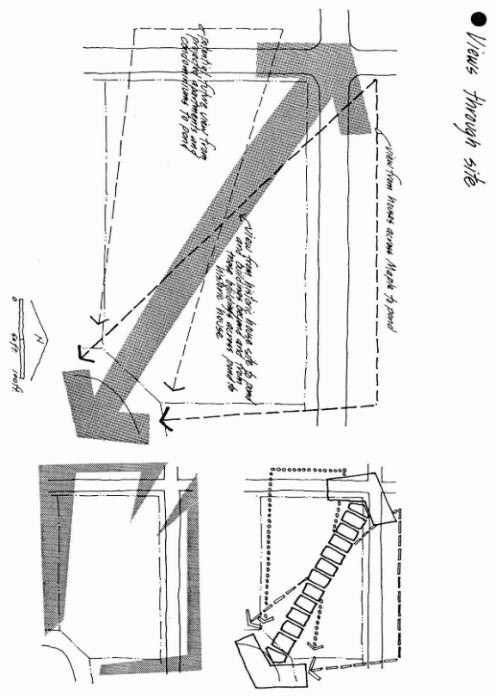
\includegraphics[width=.7\textwidth, angle=90]{../figures/views_1}
\end{frame}
\begin{frame}[mytitle=standard,t,mycolor=digiPH_gray,light]
	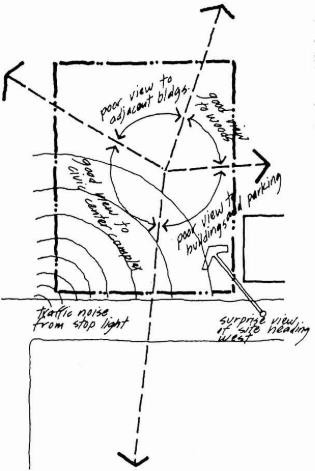
\includegraphics[width=.7\textwidth, angle=90]{../figures/views_2}
\end{frame}
\begin{frame}[mytitle=standard,t,mycolor=digiPH_gray,light]
	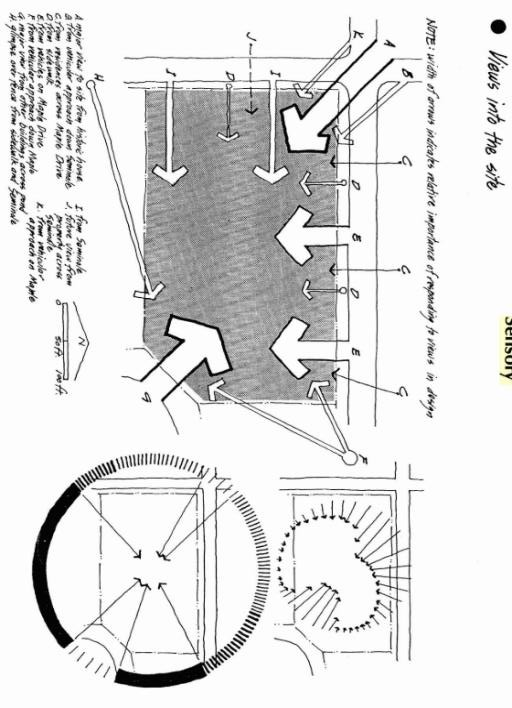
\includegraphics[width=.7\textwidth, angle=90]{../figures/views_3}
\end{frame}
\begin{frame}[mytitle=standard,t,mycolor=digiPH_gray,light]
	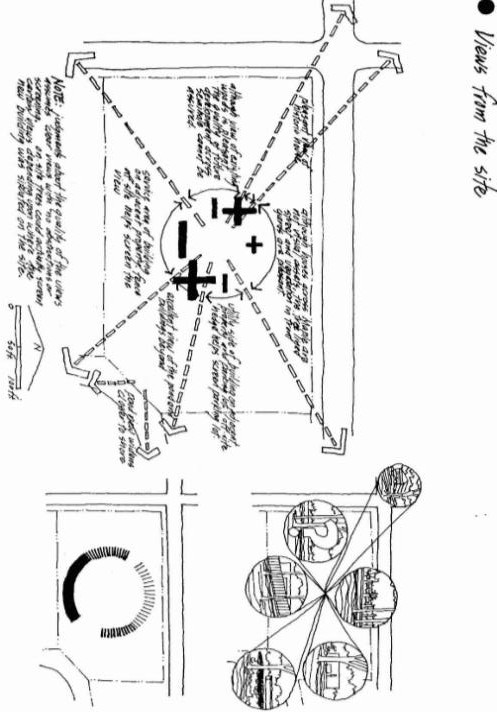
\includegraphics[width=.7\textwidth, angle=90]{../figures/views_4}
\end{frame}
\begin{frame}[mytitle=standard,t,mycolor=digiPH_gray,light]
	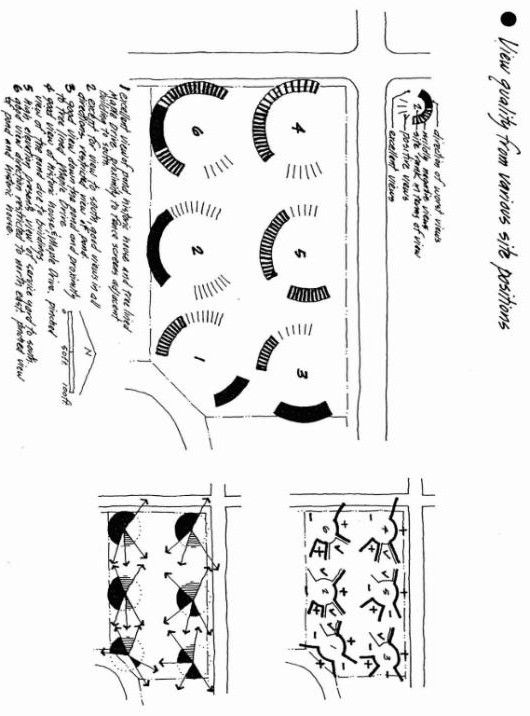
\includegraphics[width=.7\textwidth, angle=90]{../figures/views_5}
\end{frame}
\begin{frame}[mytitle=standard,t,mycolor=digiPH_gray,light]
	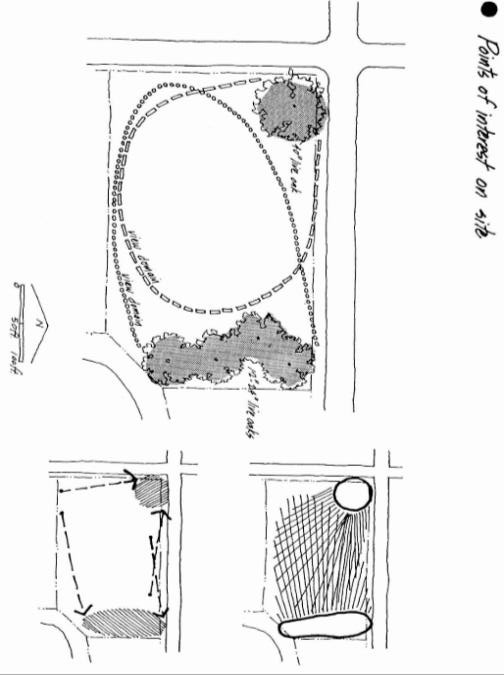
\includegraphics[width=.7\textwidth, angle=90]{../figures/views_6}
\end{frame}
% \bgdarkimg{views_7}
\bgdarkimg{view_cth}
\bgdarkimg{view_2_cth}
\bgdarkimg{view_3_cth}
\bgdarkimg{view_4_cth}
\bgdarkimg{view_kontur_regulasi_cth}


\end{document}
